\documentclass[12pt,letterpaper]{article}
\usepackage[utf8]{inputenc}
\usepackage{makeidx}
\usepackage{graphicx}
\usepackage{lmodern}
\usepackage[left=1in,right=1in,top=1in,bottom=1in]{geometry}
\raggedbottom
\author{Sean Gallagher, Hossein Hematialam, Wlodek Zadrozny}
\title{Text Mining of Medical Guidelines; Progress report for 1Q 2015}
\begin{document}

\maketitle
\begin{abstract}
Medical guidelines, which medical professionals are expected to follow, contain many conditional statements and criteria.To understand the relationship between the guidelines and results of treatments on a large scale, we need to target both for text mining. In this preliminary report we describe our preliminary results.
 
Medical guidelines text tends to be relatively regular, making it amenable to several approaches, including: 1) analysis of constituent trees, 2) regular expression matches on plain text, and 3) detecting disease-related information based on type detection. In our samples, recursive analyses of constituent parses have proven to be excessively brittle and difficult scale for many types of condition-action pairs; often nearly every sample requires another rule of analysis. A regular expression based approach has proven to be a simple, efficient solution with an average of 68.25\% precision: 62\% for Rhinosinusitis guidelines, 64\% for Hypertension guidelines, 80\% precision for Diabetes guidelines known to contain the phrase A1C, and 57\% precision for all the included Diabetes guidelines. The recall of these sets is uncertain due to the large source text size. The type-directed approach is not complete enough to create condition-action pairs, but determines the lexical types of symptoms and tests with generally perfect precision for a small sample, and a recall of 22\% and 100\% respectively. Symptoms are problematic for recall in particular due to an array of type synonyms not yet accounted for, a solution to which is among our future directions.
\end{abstract}

\section{Preprocessing}
The American Diabetes Association(ADA) publishes standards of medical cares in diabetes annually in its "Diabetes Care" journal. We consider ADA's guidelines \cite{american2013diagnosis} as our primary text source. It provides positive statements, tables, and figures about diabetes. We started by converting the guidelines from PDF to text format, editing sentences only to manage encoding errors, the majority of which were bullet points. Tables and some figures pose a problem, becoming unstructured text with many ambiguities. For example, Table 9 in our source text is replaced with a sentence of more than 80 words.

In the next step, we tried to detect sentences of the text by LingPipe sentence detector which has reasonable accuracy and recall for our project. It detected 5,532 sentences from the text. 232 sentences contain "A1C" term which is an important factor in diagnosing diabetes.
   
\section{Constituent Trees}
Our first attempt at extracting medical conditions and symptoms from unstructured text is by using hierarchical analysis of a constituent parse tree of the text. The system is relatively simple, following a general pattern:

\begin{enumerate}
\item Descend to the leaves of the tree, the original words.
\item Match classes of words for operators and numeric values.
\item Match the remaining words against known tests and diseases.
\item Ascend the tree, combining analyses as follows:
\begin{itemize}
	\item A decimal value, an operator, and a test constitute a condition.
	\item A condition and an ailment constitute a \emph{link}, which is the program output.
\end{itemize}
\end{enumerate}

There are several concerns about this approach, not the least of which are the limited scope of the links it can extract. It expects guidelines of the form
"Values of $A1C \geq 6.5$ may indicate diabetes," but this causes serious brittleness. Consider the generally equivalent statement: "A1C values predict diabetes when greater than approximately 6.5."

There are also weaknesses with tables, which are relatively common in medical literature, and any document with more then a few such links. Take for example the Wikipedia article on diabetes. The condition information is stored in a structured way, as a table. The trouble is that it is not clear how to interpret the contents. "$\geq 6.5$" can be interpreted as a operator and value. But the rest of the content needs more context, and this is what we are aiming to solve in section four.
\begin{figure}
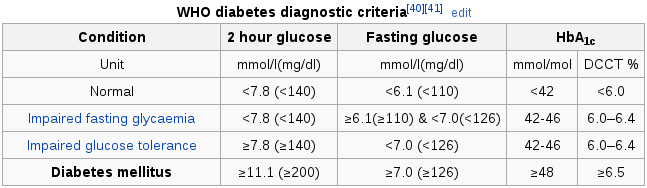
\includegraphics[width=\textwidth]{WikipediaA1CTable}
\caption{Excerpt of the Wikipedia Article on Diabetes}
\end{figure}
\section{Regular Expressions}
Modeling data is an essential part of information extraction from an unstructured data source like textual guidelines. Condition-action sentences provide information about the process flow in Clinical Guidelines. In this stage, we focus on modeling these sentences and extracting them automatically.

Condition-action sentences are not always in form of ``\texttt{if} condition \texttt{then} action''. For example, in the sentence ``Conditions that affect erythrocyte turnover and hemoglobin variants must be considered, particularly when the A1C result does not correlate with the patient's clinical situation'', we have a condition-action sentence without an ``if'' term. On the other hand, conditions may refer to effects, intentions, or events rather than activities. For instance, we see an effect of a condition in ``if the A1C is 7.0\% and a repeat result is 6.8\%, the diagnosis of diabetes is confirmed.'' We see that these sentences provide valuable information for us. So, for this stage of project, we consider them as true condition-action sentences. 

In order to identify condition-action sentences we used a simple pattern recognition, by inspiration of Wenzina and Kaiser's approach\cite{wenzina2013identifying},  by regular expressions. We consider four patterns for condition-sentences: 
\begin{itemize}
	\item `If condition, action.'
	\item `Action if condition'
	\item `When condition, action'
	\item `Action when condition'
\end{itemize}
We defined four regular expressions for these patterns respectively: 
\begin{itemize}
\item'(.*?)\textbackslash(SBAR \textbackslash(IN [Ii]f\textbackslash) (.*?) \textbackslash(, ,\textbackslash) (.*?)\textbackslash.'
\item'(.*?)\textbackslash(SBAR \textbackslash(IN [Ii]f\textbackslash) (.*?)\textbackslash. '
\item'(.*?)\textbackslash(SBAR \textbackslash(WHADVP \textbackslash(WRB [Ww]hen\textbackslash) (.*?) \textbackslash(, ,\textbackslash) (.*?)\textbackslash.'
\item'(.*?)\textbackslash(SBAR \textbackslash(WHADVP \textbackslash(WRB [Ww]hen\textbackslash) (.*?)\textbackslash. '
\end{itemize}

Figure 2 shows a comparison between Weniza and Kaiser's results and ours on Asthma guidelines.
\begin{figure}
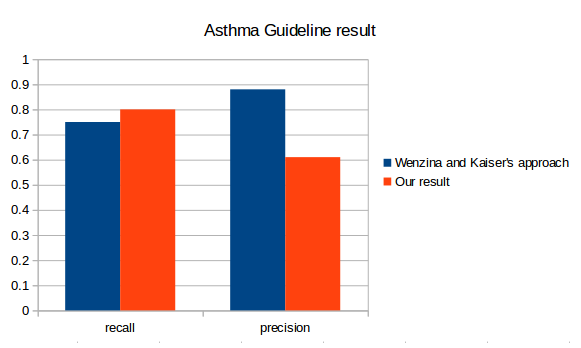
\includegraphics[width=\textwidth]{Comparison}
\caption{Comparison on Asthma Guidelines}
\end{figure}

We detected 81, 61, 62, and 60 sentences respectively, matching these patterns against the diabetes guideline. You can see some result sentences below:

\begin{itemize}
\item Sentence: ``If adults with diabetes choose to use alcohol, they should limit intake to a moderate amount (one drink per day or less for adult women and two drinks per  day or less for  adult men) and should take extra precautions to prevent hypoglycemia. (E)''

Condition: ``adults with diabetes choose to use alcohol''

Action: ``they should limit intake to a moderate amount (one drink per day or less for adult women and two drinks per day or less for adult men) and should take extra precautions to prevent hypoglycemia.''

\item Sentence: ``When people with type 1 diabetes are deprived of insulin for 12– 48 h and are ketotic, exercise can worsen hyperglycemia and ketosis (197); therefore, vigorous activity should be avoided in the presence of ketosis.''

Condition when 1: ``people with type 1 diabetes are deprived of insulin for 12 -- 48 h and are ketotic''

Action: ``exercise can worsen hyperglycemia and ketosis -LRB- 197 -RRB- ; therefore , vigorous activity should be avoided in the presence of ketosis.''

\item Sentence: ``Metformin, if not contraindicated and if tolerated, is the preferred initial pharmacological agent for type 2 diabetes. (A)''

Condition: ``tolerated''

Action: ``is the preferred initial pharmacological agent for type 2 diabetes.''
\end{itemize}

Also we found 11, 7, 2, 5 sentences with these patterns in A1C sentences. We verified these sentences and their condition and action result manually. We observed 1 error in condition determining of A1C sentences because of existence of "," in the condition part. We also observed four faults in actions. Replacing a table with a sentence and existence of "," in condition and action segments are the reason of these faults. We achieved 80\% accuracy in identifying condition-action A1C sentences. Our accuracy for the guidelines condition-action sentences is around 57\%. The decreased accuracy is the result of increasing "when" sentences, sentences with 2 conditions, sentences constructed from entire tables, and increases in sentence complexity.

We achieved 64\% and 62\% of precision in condition-action extraction of Hypertension \cite{doi:10.1001/jama.2013.284427} and Rhinosinusitis\cite{chow2012idsa} guidelines. In Rhinosinusitis guidelines, we see sentences like ''If necessary, the entire panel will reconvene to discuss potential changes.'' which lead to decrease of precision. Most of false extracted condition-action in the hypertension guidelines come from sentences those have "," in the condition part e.g. ''if pharmacologic treatment for high BP results in lower achieved SBP (eg, \textless 140 mm Hg) and treatment is well tolerated and without adverse effects on health or quality of life, treatment does not need to be adjusted.''

To solve the problem of existence of "," in the condition part, we tried to analyze parsed sentence. For example, in the sentence ''They should be stopped if no improvement in steroid dose, symptoms or lung function is detected.'', if we only try to use regular expressions, we'll get ''no improvement in steroid dose'' as a condition and ''symptoms or lung function is detected. '' as an action. But when we parse the sentence, we have the whole condition under the same parenthesis:(SBAR (IN if) (S (NP (NP (NP (DT no) (NN improvement)) (PP (IN in) (NP (NN steroid) (NN dose)))) (, ,) (NP (NP (NNS symptoms)) (CC or) (NP (NN lung) (NN function)))) (VP (VBZ is) (VP (VBN detected))))).
To achieve classification performance with regular expressions, we need to make some changes in the preprocessing stage (such as converting table sentences to a set of well structured sentences, changing passive verbs to active verbs, splitting a complex sentence to several smaller simple sentences, etc.)

\begin{figure}
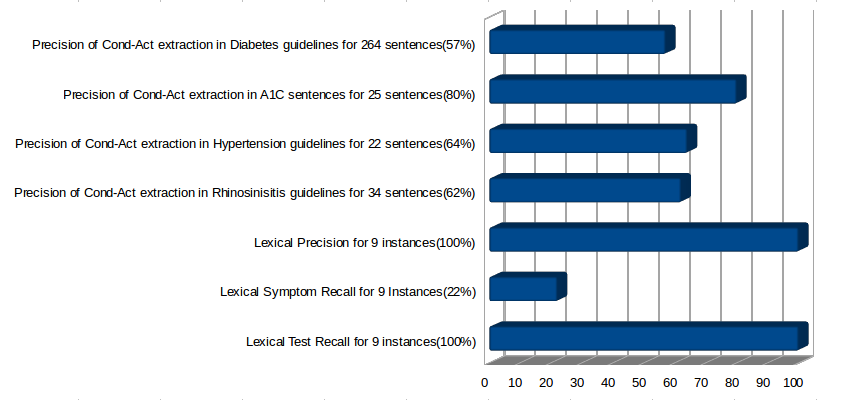
\includegraphics[width=\textwidth]{accuracies}
\caption{Accuracies of Extraction Modules (small samples)}
\end{figure}

\section{Dependency Graphs}
% Integrated into Watsonsim
We aim to improve our recognition of diagnostic criteria using other knowledge also available on Wikipedia. We can do that with many of the tools we have already been developing for question answering with Watsonsim.

Firstly, rather than hard-coding the names of many diseases we want to detect, we can recognize the types of the words we encounter using lexical type detection. This way our approach will generalize better for new diseases.
Secondly, we can use many Wikipedia sources to determine semantic relations between phrases. For example, we have determined that $HbA_{1c}$, as seen in the excerpt given above, is a synonym for the main article "Glycated hemoglobin." We do this by keeping a table of the redirects between Wikipedia articles. We also assume that phrases which label a link to an article are synonymous with the title of the target article, and we use this to measure synonymy.

\subsection{Lexical Types}
% Tried conceptnet
% Investigating NELL
On the outset we intended to use DBPedia to detect lexical types, but these are not usually specific enough to be greatly helpful, and are synonymous with the target type only on very rare occasions. We attempted to supplement this using ConceptNet, but our initial tests, before parsing the entire knowledge base, still do not indicate very high recall rates. Instead, we have developed a simple rule-based method of extracting lexical types from supporting passages. This covers many cases and the results are reasonably specific but in several instances they make unnecessary distinctions. (``Sign'' and ``symptom'' may often be used interchangably, even though Wikipedia makes a distinction; similarly for ``writer'' and ``author.'') At any rate, we are examining whether to include the NELL ontology, which does at least contain many of the phrases we are targeting.

Nonetheless, there are situations where knowing the exact type of a referent is not immediately helpful. Going back to the previous example, there is no direct statement that glycated hemoglobin is a medical test in the following passage, because it is actually the subject of an implied test of its quantity:
\begin{quote}
Glycated hemoglobin (hemoglobin A1c, HbA1c, A1C, or Hb1c; sometimes also HbA1c or HGBA1C) is a form of hemoglobin that is measured primarily to identify the average plasma glucose concentration over prolonged periods of time.
\end{quote}
This is not immediately helpful because it is not yet clear that glycated hemoglobin is the subject of any test. Unless NELL or a similar ontology has this information, some other general solution for reading such tables will need to be found, or else they may need to be handled more manually.

% Could also build an ontology from reading
\subsection{Link Expansion}
When evaluating supporting passages to discover lexical types, we have found it useful to open the search from purely verifying the type of a specific name to instead finding all of the names having a specific type. As a result, finding a the wrong object with the correct lexical type but in any supporting passage triggers the suggestion of new name. This approach tends to be helpful in situations where multiple names are defined at once, such as "Polyuria and polyphagia are symptoms of diabetes."

There is also an aspect of asymmetry in the relevance of passages. The symptom of pain is relevant enough to diabetes for authors to choose to include it, but diabetes is not relevant enough to pain for the inverse to occur. Thus, you will not find evidence linking the two in a document describing pain, so the title will generally be inaccurate for a search of symptoms, and the effect of the suggestion apparatus will be exaggerated.

The new implications of the type search has the curious effect that the text analysis pipeline operates as a tree when a detected type suggests a new name. We further stimulate this effect by then searching for type definitions among the evidence collected for the new suggested names. This adds a cycle and makes the pipeline a graph. We added a simple condition ending the cycle at three loops but typically this is not triggered, as it rather quickly finds all of the available definitions related to the original topic.

% Pull pipeline
% Mention redirects
% Real links rather than redirects

\subsection{Examples and Progress}
The dependency graph approach is not complete enough to extract full conditions, though it can find symptoms and signs. For example, a query for the symptoms of diabetes will find the source text that includes the following ten symptoms for diabetes:

\medskip
\begin{tabular}{lllll}
frequent urination & increased hunger & blurry vision & 
diabetic dermadromes & fatigue \\
increased thirst & weight loss & itchy skin & slow healing of cuts & headache  \\
\end{tabular}
\medskip

The query, which is formed to imitate Jeopardy (although this soon will not be necessary), is the following: ``This symptom indicates 
diabetes.'' The suggestion apparatus finds six symptoms, two of which are symptoms of diabetes: muscle pain and thirst.

For the closely related query ``This sign indicates diabetes,'' ``Proteinuria'' is the top result, although in this case it is read from the wiki page on the symptom rather than the disease.

The query "This test indicates diabetes" discovers A1C is a test, and also suggests "blood glucose fasting test," both of which are correct.

The current recall of the lexical type apparatus on symptoms is about 22\% for diabetes, zero for hypertension (which is fine since it does not have any to speak of), but also zero for sepsis. Sepsis has plenty of symptoms, unfortunately, they are couched in a syntax indicating that sepsis may not be the only cause.

On the other hand, the precision of recognized symptoms is very high because of the strict match rules. We integrated a more complete logic engine, and developed rules to match conjunctions, but we are uncertain how to recognize all such verbs as "includes," "indicates," "is associated with," and such syntax to improve recall without making the rules excessively verbose. 

The situation with medical tests tend to be much clearer. The $HbA_{1c}$, as well as glucose tests, the Ham test and Fehling's solution are all detected for the query ``This test indicates diabetes," along with numerous tests not mentioned on the Wikipedia diabetes article, such as a postprandial glucose test. For hypertension, it has strong support for ``blood pressure" but also includes ``pulmonary function test" and ``renal glycosuria."

\section{Software}

We used a number of software packages to develop the existing software. In particular, we used CoreNLP \cite{manning-EtAl:2014:P14-5} for constructing constituent and dependency parses, and LingPipe for additional constituent parses, which was the initial stage of our development.
We used Apache Jena and Fuzeki with TDB for interfacing with the DBPedia RDF database as part of the lexical types setup, but DBPedia ontologies provided few sufficiently specific types. We later used logic-programming style rules supported by Jena's Reasoner interface to detect types in passages, but after some limitations made processing prohibitively slow, we rewrote our lexical recognition rules for TuProlog. 

The project source code was written in a mixture of Scala and Java, according to what was more appropriate at the time. Since several of our components run independently, the language difference rarely played a role in development.

\section{Next Steps}
\subsection*{Scope}

The modules described in this paper are part of a larger scope. Our concept is to write and use several modules taking multiple approaches of information analysis of unstructured text, in order  to generate a more comprehensive and more easily searched representation of medical guidelines. When we can generate a sufficient repository of these guidelines, we have in mind to:

\begin{enumerate}
\item Make the indexed guidelines available in a way that one can determine possible remedial actions given a set of diagnostic conditions,
\item Suggest additional diagnostic criteria needed to determine a remedial action,
\item Assess the consistency of multiple guidelines and multiple sources of guidelines, with a focus on the percentage consensus for a range of possibly non-numeric values, including visualization if necessary,
\item Given the necessary level of cooperation from neighboring institutions, evaluate how existing records conform to the mined guidelines.
\end{enumerate}

\subsection*{Architecture}
Like many text analytics applications, we intend to operate using a pipeline. We have discovered the need for the following operations, which we have thus far been only partially automated:

\begin{enumerate}
\item Write a general method of reformatting incoming documents into plain text, paying special attention to tables and lists, since these contain the majority of the rules and can be otherwise very difficult to parse. Judging from the time spent on this activity in the previous months, we expect this to be the most important and difficult step.
\item Parse the resulting text, using all three of the methods mentioned above. We intend to label table cells with their column and row headers, with the understanding that these contribute usually to either the antecedents of the rules, or to the lexical type of the consequent remedies. 
\item Inject related information from existing knowledge bases where necessary in order to fill in gaps or missing context from the text. This now consists of verifying lexical types, but we target medical ontologies and thesauri in particular.
\item Filter and score condition-action rules in order to maximize precision of the results.
\end{enumerate}

\subsection*{Details}
Tables are expected to be a major bugaboo in our architecture since they have dense, semi-structured data that does not conform very well to either paradigm of analysis. We believe we can improve the quality of analysis by taking into account the row and column context. The headers may contain conditions and lexical types, but supposing these are missing or ambiguous, it may also be possible to arrive at a conclusion using the neighbors as examples. However, any ambiguity in the headers will likely be greatly magnified in the cells. Referring back to Figure 1, notice the wide array of problems such analysis faces.
\begin{enumerate}
\item 21 cells have no English text.
\item There are two rows of column-level headers, and both are necessary to make sense of the type of the cells over which they preside.
\item Two of the second-level headers define two types simultaneously, and imply a syntax used to delimit the values, as well as an equivalence between them. 
\item Each value is implicitly an interval, where in all but four cases one endpoint is implied.
\item The senses are partially reversed, and incomplete. The row-level headers are diseases, not actions, and the cell values are antecedents, also not actions. Nonetheless, since they can be used to predict diseases, which themselves can be linked with guidelines actions, they cannot be discarded as needless.
\end{enumerate}

Even existing modules have room for improvement. The dependency graphs hold promise to be used for the same extraction as the regular expression approach, but with greater flexibility in terms of syntax. It would also have available to it many other annotations and tags that regular expressions do not. Regardless of the source of the rule, we intend to use these measures for scoring the result quality.

We believe we can improve the recall of the lexical type system if we use the relations in a transitive way. For example, as it now stands, finding $HbA_{1c}$ in a list of guidelines is not sufficient to suggest it as a test. It also needs outside information, possibly found in the same search. But we believe it is tractable to detect such types from across many sources in a preprocessing step. 

\section{Conclusions}

Our project consists of several generally independent modules, and represents a foray into the possibilities of text mining for this particular domain. The current system has been shown to produce relatively precise information from plain text using only machine reading and some automated filters. As expected, recall is much more difficult to ascertain and will in any case require larger sample sizes as well as a degree of expert review. Nonetheless, we have given a simple proof-of-concept for a number of the techniques required to assemble an architecture to digest and index medical guidelines.

\bibliographystyle{plain}
\bibliography{guidelines}
\end{document}
